A comparative analysis of termination techniques for DPO graph rewriting systems, drawn from prior work~\cite{plump1995ontermination,plump2018modular,bruggink2014termination,bruggink2015proving,endrullis2024generalized_arxiv_v2,overbeek2024termination_lmcs}, is presented in Table~\ref{tab:comparison:subgraph_counting}. Our approach successfully proves termination for 14 of these systems. 
For ease of reading, many cells in Table~\ref{tab:comparison:subgraph_counting} are marked with "\textbf{$-$}", indicating that the corresponding technique is out of scope for the given example or, more often, that it is not relevant to our discussion, since other entries already show that the technique and our method are not directly comparable.

In the remainder of this section, we compare our method with some existing methods in more detail.


{% local group
  \setlength{\tabcolsep}{3pt}
  \renewcommand{\arraystretch}{1}
\begin{table}[H]
   \centering
  \small % Reduce font size
  \caption{Applicability of termination techniques to DPO rewriting examples.
  The symbol \ding{51} indicates that termination can be proved by the technique,
  \ding{55} indicates it cannot be proved, and 
  \textbf{$-$} denotes irrelevance or out-of-scope cases.
        }
 \label{tab:comparison:subgraph_counting}
% \setlength{\tabcolsep}{4pt} % Reduce horizontal padding
   \begin{NiceTabular}{ccccccccc}[vlines] % <-- 9 columns now (was 7)
    \Hline
                % \diagbox{\enskip \textbf{Examples}}{\textbf{Techniques}} 
    \Block{1-2}{\diagbox{\enskip \textbf{Examples}}{\textbf{Techniques}}} & 
    &
    \RowStyle{\rotate}
     \makecell{Forward closure \cite{plump1995ontermination}} % NEW column #1
    & \RowStyle{\rotate}
     \makecell{Modular criterion \cite{plump2018modular}} % NEW column #2
    & \RowStyle{\rotate}
     \makecell{Type graph \cite{bruggink2014termination}}  
    & \RowStyle{\rotate}
     \makecell{Type graph \cite{bruggink2015proving}} 
    & \RowStyle{\rotate}
     \makecell{Type graph \cite{endrullis2024generalized_arxiv_v2}} 
    & \RowStyle{\rotate}
     \makecell{Subgraph 
            counting \cite{overbeek2024termination_lmcs}} 
    & \RowStyle{\rotate}
     \makecell{Morphism
                Counting 
                \\(Chapter~\ref{chap:subgraph_counting})} \\
    \Hline
    \Hline
% ok examples
Chapter~\ref{chap:subgraph_counting} 
&Example~\ref{subgraph_counting:ex_contrib_variant}
  & \ding{51} & \ding{55} & \ding{55} & \ding{55} & \ding{55} & \ding{55} & \ding{51} \\ \Hline
  
\cite{plump1995ontermination} &
\hyperref[ex:overbeek_5d8_plump1995_3d8_plump2018_3_overbeek_5d8]{Example 3.8}
             & \ding{51} & -- & -- & -- & -- &
          --
             & \ding{51}\\ 
\hline

\Block{2-1}{\cite{plump2018modular}} & \hyperref[ex:overbeek_5d8_plump1995_3d8_plump2018_3_overbeek_5d8]{Example 3} 
          & -- & \ding{51} &  -- & -- & -- & 
          --
          & \ding{51}\\ 

\Hline

%~\cite{plump2018modular} 
& Example 5 &  -- &  \ding{51} &   -- & -- & -- &  
            --
          & \ding{51}\\  
\Hline

\cite{bruggink2014termination} & \hyperref[{subgraph_counting:ex:termination:bruggink14_ex4_and6}]{Examples 4 and 6}  
  & -- & -- & \ding{51} & -- & -- & 
            --
          & \ding{51} \\ \Hline

\Block{2-1}{\cite{bruggink2015proving}} & \hyperref[subgraph_counting:ex:termination:bruggink15_ex2]{Example 2}  
  & -- & -- & -- & \ding{51} & -- & 
  -- &  \ding{51}\\ \Hline
  
%~\cite{bruggink2015proving}
 & \hyperref[subgraph_counting:ex:bruggink2015_ex4]{Example 4} 
  & -- & -- & -- & \ding{51} & -- & 
  --& \ding{51} \\ \Hline


% ----- from endrullis2024generalized_arxiv_v2 -----
\Block{3-1}{\cite{endrullis2024generalized_arxiv_v2}} & \hyperref[ex:endrullis2024_6d2]{Example 6.2}  
  & -- & -- & -- & -- & \ding{51} & -- & \ding{51}\\ \Hline

%~\cite{endrullis2024generalized_arxiv_v2}
 & \hyperref[ex_endrullis_6d3_endrullis_5d8]{Example 6.3}
  & -- & -- & -- & -- & \ding{51} &% \ding{55} 
  \ding{55} & \ding{51}\\ \Hline

%~\cite{endrullis2024generalized_arxiv_v2} 
& \hyperref[ex:overbeek_5d8_plump1995_3d8_plump2018_3_overbeek_5d8]{Example D.1}
  & -- & -- & -- & -- & \ding{51} & -- & \ding{51}\\ \Hline

  \Block{4-1}{\cite{overbeek2024termination_lmcs}} & \hyperref[ex:overbeek_5d3]{Example 5.3}
  & -- & -- & -- & -- & -- & \ding{51} & \ding{51}\\ \Hline

%~\cite{overbeek2024termination_lmcs} \hyperref[ex:overbeek_5d3]{Example 5.3 monic matches}
%     & -- & -- & -- & -- & -- & \ding{51} & \ding{51}\\ \Hline
%~\cite{overbeek2024termination_lmcs} 
& \hyperref[ex:overbeek_5d5]{Example 5.5} 
  & -- & -- & -- & -- & -- & \ding{51} & \ding{51}\\ \Hline

%~\cite{overbeek2024termination_lmcs} 
& \hyperref[ex:overbeek_5d6]{Example 5.6}
  & -- & -- & -- & -- & -- & \ding{51} & \ding{51} \\ \Hline

%~\cite{overbeek2024termination_lmcs} \hyperref[ex:overbeek_5d6]{Example 5.6 bis}
%     & -- & -- & -- & -- & -- & \ding{51} & -- \\ \Hline


%~\cite{overbeek2024termination_lmcs}  
& \hyperref[ex:overbeek_5d8_plump1995_3d8_plump2018_3_overbeek_5d8]{Example 5.8}
  & -- & -- & -- & -- & -- & \ding{51} & \ding{51}\\ \Hline

      % not supported examples  
     ~\cite{plump2018modular} &  \hyperref[ex:plump2018_ex6_endrullis_d4]{Example 6} &  -- & \ding{51} & -- & -- & -- & 
      --
          & -- \\
      \Hline

\Block{3-1}{\cite{endrullis2024generalized_arxiv_v2}}
 & Example 6.4  
      & -- & -- & -- & -- & \ding{51} & -- & -- \\ \Hline

%  ~\cite{endrullis2024generalized_arxiv_v2}
  &  Example 6.5  
      & -- & -- & -- & -- &  \ding{51} & -- & -- \\ \Hline

    %  ~\cite{endrullis2024generalized_arxiv_v2}
       &\hyperref[ex:plump2018_ex6_endrullis_d4]{Example D.4} 
      & -- & -- & -- & -- & \ding{51} & -- & --\\ \Hline

   % ----- from overbeek2024termination_lmcs -----
   \Block{3-1}{\cite{overbeek2024termination_lmcs}} 
      & \hyperref[ex:overbeek:5d2:limitation]{Example 5.2}
      & -- & -- & -- & -- & -- & \ding{51} & -- \\ \Hline

    %  ~\cite{overbeek2024termination_lmcs} 
      & Example 5.7 
      & -- & -- & -- & -- & -- & \ding{51} & -- \\ \Hline
      
%  ~\cite{overbeek2024termination_lmcs} 
  & Example 5.9 
      & -- & -- & -- & -- & -- & \ding{51} & --\\ \Hline
 

    % not ok examples
   ~\cite{plump1995ontermination} & \hyperref[ex:plump95_4d1]{Example 4.1} & \ding{51} & -- & -- & -- & -- & 
              \ding{51}
              
              & \ding{55}\\ 
   \Hline
  ~\cite{plump2018modular} & \hyperref[ex:plump_ex4]{Example 4} &  -- &  \ding{51} &  -- & -- & -- & 
               --
               & \ding{55}\\ 
   \Hline

   \Block{3-1}{\cite{bruggink2014termination}} & Example 1 
   & -- & -- & \ding{51} & -- & -- & 
                 --
               &  \ding{55}\\ 
   \Hline

%   ~\cite{bruggink2014termination} 
   & Routing Protocol
       & -- & -- & \ding{51} & -- & -- & 
           --
           &  \ding{55}\\  
           \Hline
% \Block{2-1}{\cite{bruggink2014termination}}
 & \hyperref[ex:plump_ex4]{Example 5}
   & -- & -- & \ding{51} & -- & -- & -- &  \ding{55}\\ 
\Hline

\Block{2-1}{\cite{bruggink2015proving}} & \hyperref[ex:bruggink2015_ex5]{Example 5}
   & -- & -- & -- & \ding{51} & -- &  
   -- &  \ding{55}\\
   \Hline

%   ~\cite{bruggink2015proving} 
   & \hyperref[ex:bruggink2015_ex6_endrullis2024_d2]{Example 6} 
   & -- & -- & -- & \ding{51} & -- &  
   --&  \ding{55}\\  
   \Hline

   \Block{2-1}{\cite{endrullis2024generalized_arxiv_v2}} & \hyperref[ex:bruggink2015_ex6_endrullis2024_d2]{Example D.2} 
   & -- & -- & -- & -- & \ding{51} & -- & \ding{55}\\ 
   \Hline

%   ~\cite{endrullis2024generalized_arxiv_v2}
   & \hyperref[ex:endrullis:d3:limitation]{Example D.3}
   & -- & -- & -- & -- & \ding{51} & \ding{55} & \ding{55}\\ \Hline

  \end{NiceTabular}
  % \vspace{2mm}
  % \caption{Applicability of termination techniques to DPO rewriting examples.
  %  The symbol \ding{51} indicates termination can be proved by the technique,
  %  \ding{55} indicates it cannot be proved, and 
  %  $-$ denotes irrelevance or out-of-scope cases.
  %        }
  % \label{tab:comparison}
  \end{table}
} 


The subgraph counting method by Overbeek and Endrullis (2024)~\cite{overbeek2024termination_lmcs} is designed for a more general rewriting formalism capable of simulating left-injective DPO rewriting, and it can be applied to various graph notions. It is very closely related to our work in the setting where they are both defined. Both methods weigh objects by summing weighted morphisms targeting them, and, for both methods, the key challenge lies in estimating weights for morphisms whose images partially overlap with the rewriting context, because morphisms fully embedded in the context are shared between host and resulting graphs, while those entirely within left- or right-hand-side graphs are trivial to quantify.  

The two methods employ distinct strategies to overcome this challenge. The subgraph counting method relies on type-morphisms (see~\cite[page 9, remark 4.11, Lemma 4.23]{overbeek2024termination_lmcs}), whereas our approach requires injective mappings from (i) subgraph occurrences partially overlapping the rewriting context in the result graph to (ii) those in the host graph.

Both approaches have limitations and strengths. Endrullis and Overbeek's approach suffers from discrete interfaces\textemdash{}interface graphs with no edges, as mentioned in~\cite[Example 5.5]{overbeek2024termination_lmcs}. For instance, it proves termination of Example~\ref{ex:overbeek_5d5}:
\begin{center}
      \resizebox{0.9\textwidth}{!}{
          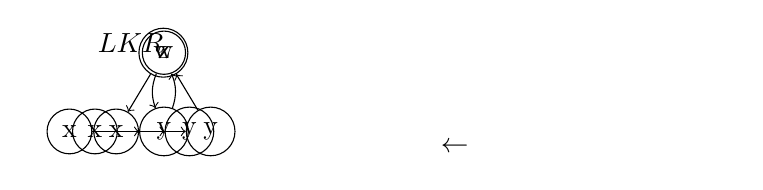
\begin{tikzpicture}
              \graphbox{$L$}{0mm}{0mm}{35mm}{25mm}{2mm}{-8mm}{
                  \coordinate (delta) at (0,-18mm);
                  \node[draw,circle] (x) at (-6mm,-10mm) {x};
                  \node[draw,circle] (y) at (6mm,-10mm) {y};
                  \node[draw,circle]  (z) at (6mm,0mm) {z};
                  \draw[->]  (x) to (y);
                  \draw[->] (y) to[bend right=20] (z);
                  \draw[->]  (z) to[bend right=20] (y);
              }
              \graphbox{$K$}{40mm}{0mm}{35mm}{25mm}{2mm}{-8mm}{
                  \node[draw,circle]  (x) at (-6mm,-10mm) {x};
                  \node[draw,circle]  (y) at (6mm,-10mm) {y};
                  \draw[->] (x) to (y);
              }
              \graphbox{$R$}{80mm}{0mm}{35mm}{25mm}{2mm}{-8mm}{
                  \node[draw,circle]  (x) at (-6mm,-10mm) {x};
                      \node[draw,circle]  (y) at (6mm,-10mm) {y};
                      \node[draw,circle]  (z) at (0mm,0mm) {w};
                      \draw[->]  (x) to (y);
                      \draw[->]  (y) to [bend left=0] (z);
                      \draw[->]  (z) to [bend left=0] (x);
              }
              \node () at (37mm,-12mm) {$\leftarrow$};
              \node () at (78mm,-12mm) {$\rightarrow$};
          \end{tikzpicture}
      }
  \end{center}
   but fails for Example~\ref{ex_endrullis_6d3_endrullis_5d8}:
   \begin{center}
    \resizebox{0.9\textwidth}{!}{
          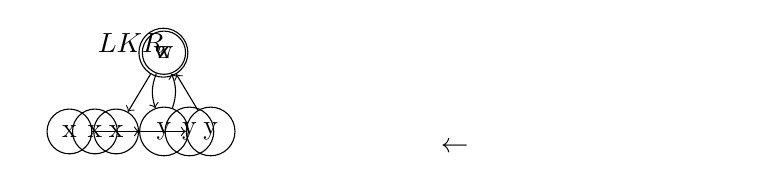
\begin{tikzpicture}
              \graphbox{$L$}{0mm}{0mm}{35mm}{25mm}{2mm}{-8mm}{
                  \coordinate (delta) at (0,-18mm);
                  \node[draw,circle] (x) at (-6mm,-10mm) {x};
                  \node[draw,circle] (y) at (6mm,-10mm) {y};
                  \node[draw,circle]  (z) at (6mm,0mm) {z};
                  \draw[->]  (x) to (y);
                  \draw[->] (y) to[bend right=20] (z);
                  \draw[->]  (z) to[bend right=20] (y);
              }
              \graphbox{$K$}{40mm}{0mm}{35mm}{25mm}{2mm}{-8mm}{
                  \node[draw,circle]  (x) at (-6mm,-10mm) {x};
                  \node[draw,circle]  (y) at (6mm,-10mm) {y};
              }
              \graphbox{$R$}{80mm}{0mm}{35mm}{25mm}{2mm}{-8mm}{
                  \node[draw,circle]  (x) at (-6mm,-10mm) {x};
                      \node[draw,circle]  (y) at (6mm,-10mm) {y};
                      \node[draw,circle]  (z) at (0mm,0mm) {w};
                      \draw[->]  (x) to (y);
                      \draw[->]  (y) to [bend left=0] (z);
                      \draw[->]  (z) to [bend left=0] (x);
              }
              \node () at (37mm,-12mm) {$\leftarrow$};
              \node () at (78mm,-12mm) {$\rightarrow$};
          \end{tikzpicture}
    }
  \end{center}
% ~\cite[Example 6.3]{endrullis2024generalized_arxiv_v2}
However, the two rules differ only by an edge in the interface graph.
Similarly, it fails to prove termination for Example~\ref{subgraph_counting:ex_contrib_variant}:
 \begin{center}
  \resizebox{0.9\textwidth}{!}{
            \begin{tikzpicture}
                \graphbox{$L$}{0mm}{0mm}{35mm}{37mm}{2mm}{-5mm}{
                    \coordinate (delta) at (0,-18mm);
                    \node[draw,circle] (l1) at ($(delta)+(-1,1.5)$) {$1$};
                    \node[draw,circle] (l2) at ($(delta)+(1,1.5)$) {$2$};
                    \node[draw,circle] (l3) at ($(delta)+(0,0)$) {3};
                    \draw[->] (l1) -- (l3) node[midway,left] {$s$};
                    \draw[->] (l2) -- (l3) node[midway,right] {$s$};
                    \draw[->] (l3) edge [loop below] node {$0$} (l3);
                }
                \graphbox{$K$}{40mm}{0mm}{35mm}{37mm}{2mm}{-5mm}{
                    \coordinate (delta) at (0,-18mm);
                    \coordinate (interfaceorigin) at ($(delta) +(5,0)$);
                    \node[draw,circle] (r1) at ($(delta) +(-1,1.5)$) {$1$};
                    \node[draw,circle] (r2) at ($(delta) +(0.5,1.5)$) {$2$};
                    \node[draw,circle] (r3) at ($(delta)+(0,0)$) {3};
                    % \draw[->] (r1) -- (r3) node[midway,left] {$s$};
                    % \draw[->] (r3) edge [loop below] node {$0$} (r3);
                }
                \graphbox{$R$}{80mm}{0mm}{50mm}{37mm}{2mm}{-5mm}{
                    \coordinate (delta) at (-10mm,-18mm);
                    \node[draw,circle] (r1) at ($(delta)+(-1,1.5)$) {$1$};
                    \node[draw,circle] (r2) at ($(delta)+(0.5,1.5)$) {$2$};
                    \node[draw,circle] (r3) at ($(delta)+(0,0)$) {3};
                    \node[draw,circle] (r4) at ($(delta)+(1,0)$) {4};
                    \draw[->] (r1) -- (r3) node[midway,left] {$s$};
                    \draw[->] (r2) -- (r4) node[midway,right] {$s$};
                    \draw[->] (r4) edge [loop below] node {$0$} (r4);
                    \draw[->] (r3) edge [loop below] node {$0$} (r3);
                    \node[draw,circle] (r5) at ($(r2)+(1.5,0)$) {};
                    \draw[->] (r5) edge [loop below] node {$0$} (r5);
                    \draw[->] (r5) edge [loop right] node {$0$} (r5);
                    \draw[->] (r5) edge [loop left] node {$0$} (r5);
                }
                \node () at (38mm,-18mm) {$\leftarrow$};
                \node () at (77mm,-18mm) {$\rightarrow$};
            \end{tikzpicture}
      } 
    \end{center}
    However, it succeeds if if an edge labeled by ``s'' from node $1$ to node $3$ is added to the interface graph. Our approach, however, can handle all the aforementioned cases. Nevertheless, their method can address the system in Example~\ref{ex:plump95_4d1}:
        \begin{center}
    $\rho'\mathop{=}$\scalebox{0.9} { {
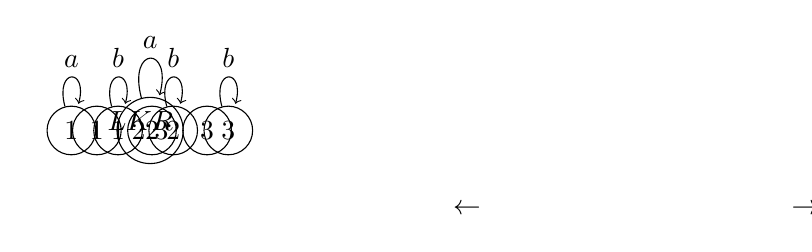
\begin{tikzpicture}[baseline=-10mm]
    \graphbox{$L$}{0mm}{0mm}{38mm}{20mm}{2mm}{-13mm}{
      \node [draw, circle] (x) at (-7mm,0mm) {1};
      \node [draw, circle] (y) at (3mm,0mm) {2 3};
      \draw[->] (x) edge[loop above] node  {$a$} (x);
      \draw[->] (y) edge [loop above] node {$a$} (y);
    }
    \graphbox{$K$}{42mm}{-0mm}{38mm}{20mm}{0mm}{-10mm}{
        \node [draw, circle] (x) at (-7mm,0mm) {1};
        \node [draw, circle] (y) at (0mm,0mm) {2};
        \node [draw, circle] (z) at (7mm,0mm) {3};    
    }
    \begin{scope}[opacity=1]        
    \graphbox{$R$}{85mm}{-0mm}{38mm}{20mm}{2mm}{-13mm}{
      \node [draw, circle] (x) at (-7mm,0mm) {1};
      \node [draw, circle] (y) at (0mm,0mm) {2};
      \node [draw, circle] (z) at (7mm,0mm) {3};
      \draw[->] (x) edge[loop above] node  {$b$} (x);
      \draw[->] (y) edge[loop above] node  {$b$} (y);
      \draw[->] (z) edge[loop above] node  {$b$} (z);
    }
    \end{scope}
    \node () at (40mm,-10mm) {$\leftarrow$};
    \node () at (83mm,-10mm) {$\rightarrow$};
\end{tikzpicture}
}

}
    % \caption{}
    % \label{fig:subgraph_counting:ex_overbeek_5d6_bis}
  \end{center} 
% (~\cite[\hyperref[ex:plump95_4d1]{Example 4.1}]{plump1995ontermination}) 
which remains beyond the scope of our technique. Finally, both approaches cannot handle Example~\ref{ex:endrullis:d3:limitation} (see~\cite[Remark 6.2]{overbeek2024termination_lmcs}).

The type graph method~\cite{zantema2014termination,bruggink2014termination,bruggink2015proving,endrullis2024generalized_icgt} is also related to our approach, as both methods involve counting morphisms. However, they differ in direction: the type graph method counts morphisms from the object to a fixed type graph, while our method counts morphisms from a fixed pattern graph to the object.
Concerning their applicability, neither method strictly subsumes the other.
On the one hand, the termination of Example~\ref{subgraph_counting:ex_contrib_variant}, shown below, can be proved by our method but not by the type graph methods due to the existence of a surjection from the output graph to the input graph as explained in~\cite[Example D.4]{endrullis2024generalized_arxiv_v2}.
\begin{center}
  \resizebox{0.9\textwidth}{!}{
            \begin{tikzpicture} 
                \graphbox{$L$}{0mm}{0mm}{35mm}{37mm}{2mm}{-5mm}{
                    \coordinate (delta) at (0,-18mm);
                    \node[draw,circle] (l1) at ($(delta)+(-1,1.5)$) {$1$};
                    \node[draw,circle] (l2) at ($(delta)+(1,1.5)$) {$2$};
                    \node[draw,circle] (l3) at ($(delta)+(0,0)$) {3};
                    \draw[->] (l1) -- (l3) node[midway,left] {$s$};
                    \draw[->] (l2) -- (l3) node[midway,right] {$s$};
                    \draw[->] (l3) edge [loop below] node {$0$} (l3);
                }
                \graphbox{$K$}{40mm}{0mm}{35mm}{37mm}{2mm}{-5mm}{
                    \coordinate (delta) at (0,-18mm);
                    \coordinate (interfaceorigin) at ($(delta) +(5,0)$);
                    \node[draw,circle] (r1) at ($(delta) +(-1,1.5)$) {$1$};
                    \node[draw,circle] (r2) at ($(delta) +(0.5,1.5)$) {$2$};
                    \node[draw,circle] (r3) at ($(delta)+(0,0)$) {3};
                    % \draw[->] (r1) -- (r3) node[midway,left] {$s$};
                    % \draw[->] (r3) edge [loop below] node {$0$} (r3);
                }
                \graphbox{$R$}{80mm}{0mm}{50mm}{37mm}{2mm}{-5mm}{
                    \coordinate (delta) at (-10mm,-18mm);
                    \node[draw,circle] (r1) at ($(delta)+(-1,1.5)$) {$1$};
                    \node[draw,circle] (r2) at ($(delta)+(0.5,1.5)$) {$2$};
                    \node[draw,circle] (r3) at ($(delta)+(0,0)$) {3};
                    \node[draw,circle] (r4) at ($(delta)+(1,0)$) {4};
                    \draw[->] (r1) -- (r3) node[midway,left] {$s$};
                    \draw[->] (r2) -- (r4) node[midway,right] {$s$};
                    \draw[->] (r4) edge [loop below] node {$0$} (r4);
                    \draw[->] (r3) edge [loop below] node {$0$} (r3);
                    \node[draw,circle] (r5) at ($(r2)+(1.5,0)$) {};
                    \draw[->] (r5) edge [loop below] node {$0$} (r5);
                    \draw[->] (r5) edge [loop right] node {$0$} (r5);
                    \draw[->] (r5) edge [loop left] node {$0$} (r5);
                }
                \node () at (38mm,-18mm) {$\leftarrow$};
                \node () at (77mm,-18mm) {$\rightarrow$};
            \end{tikzpicture}
  }
          \end{center}
        On the other hand, our method cannot prove the termination of Example~\ref{ex:endrullis:d3:limitation}, shown below, because of the injection from the left-hand side graph $L$ to the right-hand side graph $R$, but the type graph methods can handle it.
    \begin{center}
      \resizebox{0.9\textwidth}{!}{
        \begin{tikzpicture}  
          \graphbox{$L$}{0mm}{-11mm}{32mm}{15mm}{2mm}{-8mm}{  
              \node[draw,circle]  (x) at (-6mm,0mm) {$1$};  
              \node[draw,circle]  (y) at (6mm,0mm) {};  
            }  
            \graphbox{$K$}{36mm}{-11mm}{32mm}{15mm}{2mm}{-8mm}{  
              \node[draw,circle]  (x) at (-6mm,0mm) {$1$};  
            }  
            \graphbox{$R$}{72mm}{-11mm}{32mm}{15mm}{1mm}{-8mm}{  
              \node[draw,circle]  (x) at (-6mm,0mm) {$1$};  
              \node[draw,circle]  (y) at (6mm,0mm) {};  
              \draw[->]  (x) to (y);  
            }    
              \node () at (34mm,-19mm) {$\leftarrow$};
              \node () at (70mm,-19mm) {$\rightarrow$};
      \end{tikzpicture}
      }
    \end{center}
          %  On the other hand, our method cannot prove the termination of~\cite[Example 1, 5 and Ad-hoc Routing Protocol]{bruggink2014termination}, nor~\cite[Example 5, 6]{bruggink2015proving}, nor~\cite[Examples D2 and D3]{endrullis2024generalized_arxiv_v2}.

Plump (1995)~\cite{plump1995ontermination} gives a necessary and sufficient termination criterion for left-injective DPO hypergraph rewriting in terms of forward closure. However, the verification of the criterion is undecidable in general.

Our method complements the approach proposed by Plump (2018)~\cite{plump2018modular}: whereas the method decomposes a rewriting system into subsystems and proves termination of the entire system by combining termination proofs for the subsystems, the termination of each subsystem must still be established separately.
For example, the measure based on the indegree proposed in~\cite{plump2018modular} cannot prove the termination of Example~\ref{subgraph_counting:ex_contrib_variant}, illustrated below, due to the loops on the node $5$ in the right-hand side graph $R$. 
\begin{center}
  \resizebox{0.9\textwidth}{!}{
            \begin{tikzpicture} 
                \graphbox{$L$}{0mm}{0mm}{35mm}{37mm}{2mm}{-5mm}{
                    \coordinate (delta) at (0,-18mm);
                    \node[draw,circle] (l1) at ($(delta)+(-1,1.5)$) {$1$};
                    \node[draw,circle] (l2) at ($(delta)+(1,1.5)$) {$2$};
                    \node[draw,circle] (l3) at ($(delta)+(0,0)$) {3};
                    \draw[->] (l1) -- (l3) node[midway,left] {$s$};
                    \draw[->] (l2) -- (l3) node[midway,right] {$s$};
                    \draw[->] (l3) edge [loop below] node {$0$} (l3);
                }
                \graphbox{$K$}{40mm}{0mm}{35mm}{37mm}{2mm}{-5mm}{
                    \coordinate (delta) at (0,-18mm);
                    \coordinate (interfaceorigin) at ($(delta) +(5,0)$);
                    \node[draw,circle] (r1) at ($(delta) +(-1,1.5)$) {$1$};
                    \node[draw,circle] (r2) at ($(delta) +(0.5,1.5)$) {$2$};
                    \node[draw,circle] (r3) at ($(delta)+(0,0)$) {3};
                    % \draw[->] (r1) -- (r3) node[midway,left] {$s$};
                    % \draw[->] (r3) edge [loop below] node {$0$} (r3);
                }
                \graphbox{$R$}{80mm}{0mm}{50mm}{37mm}{2mm}{-5mm}{
                    \coordinate (delta) at (-10mm,-18mm);
                    \node[draw,circle] (r1) at ($(delta)+(-1,1.5)$) {$1$};
                    \node[draw,circle] (r2) at ($(delta)+(0.5,1.5)$) {$2$};
                    \node[draw,circle] (r3) at ($(delta)+(0,0)$) {$3$};
                    \node[draw,circle] (r4) at ($(delta)+(1,0)$) {$4$};
                    \draw[->] (r1) -- (r3) node[midway,left] {$s$};
                    \draw[->] (r2) -- (r4) node[midway,right] {$s$};
                    \draw[->] (r4) edge [loop below] node {$0$} (r4);
                    \draw[->] (r3) edge [loop below] node {$0$} (r3);
                    \node[draw,circle] (r5) at ($(r2)+(1.5,0)$) {5};
                    \draw[->] (r5) edge [loop below] node {$0$} (r5);
                    \draw[->] (r5) edge [loop right] node {$0$} (r5);
                    \draw[->] (r5) edge [loop left] node {$0$} (r5);
                }
                \node () at (38mm,-18mm) {$\leftarrow$};
                \node () at (77mm,-18mm) {$\rightarrow$};
            \end{tikzpicture}
  }
          \end{center}
Specifically, consider the following rewriting step using the rule:
\begin{center}
  \resizebox{0.7\textwidth}{!}{
            \begin{tikzpicture}
                \graphbox{$G$}{0mm}{0mm}{35mm}{37mm}{2mm}{-5mm}{
                    \coordinate (delta) at (0,-18mm);
                    \node[draw,circle] (l1) at ($(delta)+(-1,1.5)$) {$1$};
                    \node[draw,circle] (l2) at ($(delta)+(1,1.5)$) {$2$};
                    \node[draw,circle] (l3) at ($(delta)+(0,0)$) {3};
                    \draw[->] (l1) -- (l3) node[midway,left] {$s$};
                    \draw[->] (l2) -- (l3) node[midway,right] {$s$};
                    \draw[->] (l3) edge [loop below] node {$0$} (l3);
                }
                \graphbox{$H$}{40mm}{0mm}{50mm}{37mm}{2mm}{-5mm}{
                    \coordinate (delta) at (-10mm,-18mm);
                    \node[draw,circle] (r1) at ($(delta)+(-1,1.5)$) {$1$};
                    \node[draw,circle] (r2) at ($(delta)+(0.5,1.5)$) {$2$};
                    \node[draw,circle] (r3) at ($(delta)+(0,0)$) {$3$};
                    \node[draw,circle] (r4) at ($(delta)+(1,0)$) {$4$};
                    \draw[->] (r1) -- (r3) node[midway,left] {$s$};
                    \draw[->] (r2) -- (r4) node[midway,right] {$s$};
                    \draw[->] (r4) edge [loop below] node {$0$} (r4);
                    \draw[->] (r3) edge [loop below] node {$0$} (r3);
                    \node[draw,circle] (r5) at ($(r2)+(1.5,0)$) {5};
                    \draw[->] (r5) edge [loop below] node {$0$} (r5);
                    \draw[->] (r5) edge [loop right] node {$0$} (r5);
                    \draw[->] (r5) edge [loop left] node {$0$} (r5);
                }
                \node () at (38mm,-18mm) {$\Rightarrow$};
            \end{tikzpicture}
  }
          \end{center}
For all $k \mathop{\in} \mathbb{N}$, the weight of the host graph $G$\textemdash{}defined as the sum of node indegrees raised to the power of $k$\textemdash{}is $0^k + 0^k + 3^k = 3^k$, while the weight of the result graph $H$ is $0^k + 0^k + 2^k + 2^k + 3^k = 2^k + 2^k + 3^k$. Since $3^k < 2^k + 2^k + 3^k$, the weight does not decrease. However, our method succeeds (see Example~\ref{subgraph_counting:ex_contrib_variant}).



